\documentclass[11pt]{article}

\usepackage{amsmath,amssymb,amsfonts}
\usepackage{graphicx}
\usepackage{pgfplots}
\usepackage{multicol}
\usepackage{enumitem}
\usepgfplotslibrary{fillbetween}
\pgfplotsset{compat=1.16,width=10cm}


\setlength{\topmargin}{-.5in} \setlength{\textheight}{9.25in}
\setlength{\oddsidemargin}{0in} \setlength{\textwidth}{6.8in}


\begin{document}

\Large

\noindent{\bf Name: \hfill Date: \hfill Quiz 4 \hfill AP Calculus - Hargus}

\medskip\hrule
\vspace{10pt}

\noindent \textbf{Instructions:} Please \textbf{show all work} (partial credit may be awarded for correct work, even if your answer is wrong). 

\begin{enumerate}

\item (15 points) Evaluate the \textbf{indefinite} integral using $u$-substitution. \textbf{You must show the steps of using $u$-substitution to get credit}.
\begin{enumerate}[itemsep=60pt]
    \item $\displaystyle \int \cos(2\theta+4) d\theta$
    \item $\displaystyle \int  \frac{x}{1-25x^2} dx$
    \item $\displaystyle \int x \cdot e^{x^2} dx$
\end{enumerate}

\vspace{70pt}

\item (10 points) Evaluate the \textbf{definite} integral using $u$-substitution. \textbf{You must show the steps of using $u$-substitution to get credit}.
\begin{enumerate}[itemsep=60pt]
    \item $\displaystyle \int_{1}^{2} x^2 (x^3 - 1)^4 dx$
    \item $\displaystyle \int_{0}^{1} \ln(2) \cdot 2^{x+3} dx$
\end{enumerate}

\newpage

\item (10 points) Find the average value of $f(x) = x^3$ between $x=0$ and $x=2$
\vspace{100pt}

\item (10 points) Let $f(x)$ be a differentiable function for which $f'(x)=3f(x)$.
\begin{enumerate}
    \item $f(x)$ is which kind of function? (choose one)
\begin{enumerate}
    \item Quadratic
    \item Exponential
    \item Cosine
\end{enumerate}
    \item Write an equation for $f(x)$, if $f(0)=5$.
\end{enumerate}

\vspace{70pt}


\item (15 points) Write an expression for the gray area below between $y=\frac{1}{x}$ and $y=\frac{1}{2}$ from $x=1$ to $x=3$. \textbf{Write your answer using integrals, you do not need to solve the integrals}.

\begin{center}
\begin{tikzpicture}[declare function={a=1;b=3;f(\x)=1/\x;g(\x)=0.5;}]
 \begin{axis}[axis lines=middle,axis on top,xlabel=$x$,ylabel=$y$,
 xmin=-0.5,xmax=5,ymin=-0.5,ymax=2,ytick=\empty,
 xtick={a,2,b},xticklabels={$1$,$2$,$3$}, 
 every axis x label/.style={at={(current axis.right of origin)},anchor=north west},
 every axis y label/.style={at={(current axis.above origin)},anchor=north east}]
  \addplot[name path=A,blue,thick,domain=0.2:5,smooth,] {f(x)}
  node [pos=0.4, right] {$y=\frac{1}{x}$};
  \addplot[name path=B,purple,thick,domain=0.2:5,smooth] {g(x)}
  node [pos=0.8, above] {$y=\frac{1}{2}$};
  \path[name path=C] (\pgfkeysvalueof{/pgfplots/xmin},0) -- (\pgfkeysvalueof{/pgfplots/xmax},0);
    \addplot [gray] fill between [
        of=A and B,soft clip={domain=1:b},
    ];
 \end{axis}
\end{tikzpicture}
\end{center}

\vspace{20pt}

\begin{center}
Area= $\rule{10cm}{0.4pt}$
\end{center}

\newpage

\item (20 points) Answer each of the following questions by writing the correct integral. You \textbf{do} need to find the endpoints $a$ and $b$ for each integral $\int_{a}^{b}$.  You \textbf{do not} need to solve the integrals.

\begin{enumerate}[itemsep=70pt]
    \item What is the area of the gray region between the functions below?
    \item What is the volume of the object made by rotating the gray area around the $x$-axis?
    \item What is the volume of the object made by rotating the gray area around the line $x=1$?
\end{enumerate}

\vspace{70pt}

\begin{center}
\begin{tikzpicture}[declare function={a=1;b=3;f(\x)=x^2-2*x+3;g(\x)=-x^2+4*x+3;}]
 \begin{axis}[axis lines=middle,axis on top,xlabel=$x$,ylabel=$y$,
 xmin=-2,xmax=4,ymin=-0.5,ymax=10,ytick=\empty,
 xtick=\empty,, 
 every axis x label/.style={at={(current axis.right of origin)},anchor=north west},
 every axis y label/.style={at={(current axis.above origin)},anchor=north east}]
  \addplot[name path=A,blue,thick,domain=-2:5,smooth,] {f(x)}
  node [pos=0.38, below] {$y=x^2-2x+3$};
  \addplot[name path=B,purple,thick,domain=-2:5,smooth] {g(x)}
  node [pos=0.63, above] {$y=-x^2+4x+3$};
  \path[name path=C] (\pgfkeysvalueof{/pgfplots/xmin},0) -- (\pgfkeysvalueof{/pgfplots/xmax},0);
    \addplot [gray] fill between [
        of=A and B,soft clip={domain=0:b},
    ];
 \end{axis}
\end{tikzpicture}
\end{center}

\newpage

\item (\textbf{Extra Credit: 10 points}) A solid has a base inside the circle $x^2 + y^2 = 16$. The cross sections perpendicular to the x-axis are triangles with height equal to 3 times the base. Write an integral for the volume of the solid and solve to find this volume.

\end{enumerate}

\end{document} 